\documentclass[a4paper]{article}

\def\npart {III}
\def\nterm {Lent}
\def\nyear {2018}
\def\nlecturer {M.\ E.\ Cates}
\def\ncourse {Theoretical Physics of Soft Condensed Matter}

% Imports
\ifx \nextra \undefined
  \usepackage[pdftex,
    hidelinks,
    pdfauthor={Dexter Chua},
    pdfsubject={Cambridge Maths Notes: Part \npart\ - \ncourse},
    pdftitle={Part \npart\ - \ncourse},
  pdfkeywords={Cambridge Mathematics Maths Math \npart\ \nterm\ \nyear\ \ncourse}]{hyperref}
  \title{Part \npart\ - \ncourse}
\else
  \usepackage[pdftex,
    hidelinks,
    pdfauthor={Dexter Chua},
    pdfsubject={Cambridge Maths Notes: Part \npart\ - \ncourse\ (\nextra)},
    pdftitle={Part \npart\ - \ncourse\ (\nextra)},
  pdfkeywords={Cambridge Mathematics Maths Math \npart\ \nterm\ \nyear\ \ncourse\ \nextra}]{hyperref}

  \title{Part \npart\ - \ncourse \\ {\Large \nextra}}
\fi

\author{Lectured by \nlecturer \\\small Notes taken by Dexter Chua}
\date{\nterm\ \nyear}

\usepackage{alltt}
\usepackage{amsfonts}
\usepackage{amsmath}
\usepackage{amssymb}
\usepackage{amsthm}
\usepackage{booktabs}
\usepackage{caption}
\usepackage{enumitem}
\usepackage{fancyhdr}
\usepackage{graphicx}
\usepackage{mathtools}
\usepackage{microtype}
\usepackage{multirow}
\usepackage{pdflscape}
\usepackage{pgfplots}
\usepackage{siunitx}
\usepackage{tabularx}
\usepackage{tikz}
\usepackage{tkz-euclide}
\usepackage[normalem]{ulem}
\usepackage[all]{xy}

\pgfplotsset{compat=1.12}

\pagestyle{fancyplain}
\lhead{\emph{\nouppercase{\leftmark}}}
\ifx \nextra \undefined
  \rhead{
    \ifnum\thepage=1
    \else
      \npart\ \ncourse
    \fi}
\else
  \rhead{
    \ifnum\thepage=1
    \else
      \npart\ \ncourse\ (\nextra)
    \fi}
\fi
\usetikzlibrary{arrows}
\usetikzlibrary{decorations.markings}
\usetikzlibrary{decorations.pathmorphing}
\usetikzlibrary{positioning}
\usetikzlibrary{fadings}
\usetikzlibrary{intersections}
\usetikzlibrary{cd}

\newcommand*{\Cdot}{\raisebox{-0.25ex}{\scalebox{1.5}{$\cdot$}}}
\newcommand {\pd}[2][ ]{
  \ifx #1 { }
    \frac{\partial}{\partial #2}
  \else
    \frac{\partial^{#1}}{\partial #2^{#1}}
  \fi
}

% Theorems
\theoremstyle{definition}
\newtheorem*{aim}{Aim}
\newtheorem*{axiom}{Axiom}
\newtheorem*{claim}{Claim}
\newtheorem*{cor}{Corollary}
\newtheorem*{defi}{Definition}
\newtheorem*{eg}{Example}
\newtheorem*{fact}{Fact}
\newtheorem*{law}{Law}
\newtheorem*{lemma}{Lemma}
\newtheorem*{notation}{Notation}
\newtheorem*{prop}{Proposition}
\newtheorem*{thm}{Theorem}

\renewcommand{\labelitemi}{--}
\renewcommand{\labelitemii}{$\circ$}
\renewcommand{\labelenumi}{(\roman{*})}

\let\stdsection\section
\renewcommand\section{\newpage\stdsection}

% Strike through
\def\st{\bgroup \ULdepth=-.55ex \ULset}

% Maths symbols
\newcommand{\bra}{\langle}
\newcommand{\ket}{\rangle}

\newcommand{\N}{\mathbb{N}}
\newcommand{\Z}{\mathbb{Z}}
\newcommand{\Q}{\mathbb{Q}}
\renewcommand{\H}{\mathbb{H}}
\newcommand{\R}{\mathbb{R}}
\newcommand{\C}{\mathbb{C}}
\newcommand{\Prob}{\mathbb{P}}
\renewcommand{\P}{\mathbb{P}}
\newcommand{\E}{\mathbb{E}}
\newcommand{\F}{\mathbb{F}}
\newcommand{\cU}{\mathcal{U}}
\newcommand{\RP}{\mathbb{RP}}
\newcommand{\CP}{\mathbb{CP}}

\newcommand{\ph}{\,\cdot\,}

\DeclareMathOperator{\sech}{sech}
\DeclareMathOperator{\cosech}{cosech}
\DeclareMathOperator{\cosec}{cosec}

\DeclareMathOperator{\covol}{covol}
\DeclareMathOperator{\vol}{vol}

\let\Im\relax
\let\Re\relax
\DeclareMathOperator{\Im}{Im}
\DeclareMathOperator{\Re}{Re}
\DeclareMathOperator{\im}{im}
\DeclareMathOperator{\image}{image}
\DeclareMathOperator{\Ann}{Ann}

\DeclareMathOperator*{\res}{res}
\DeclareMathOperator{\Res}{Res}
\DeclareMathOperator{\Ind}{Ind}

\DeclareMathOperator{\tr}{tr}
\DeclareMathOperator{\diag}{diag}
\DeclareMathOperator{\rank}{rank}
\DeclareMathOperator{\card}{card}
\DeclareMathOperator{\spn}{span}
\DeclareMathOperator{\adj}{adj}

\DeclareMathOperator{\erf}{erf}
\DeclareMathOperator{\erfc}{erfc}

\DeclareMathOperator{\ord}{ord}
\DeclareMathOperator{\Sym}{Sym}

\DeclareMathOperator{\sgn}{sgn}
\DeclareMathOperator{\orb}{orb}
\DeclareMathOperator{\stab}{stab}
\DeclareMathOperator{\ccl}{ccl}

\DeclareMathOperator{\lcm}{lcm}
\DeclareMathOperator{\hcf}{hcf}

\DeclareMathOperator{\Int}{Int}
\DeclareMathOperator{\id}{id}

\DeclareMathOperator{\betaD}{beta}
\DeclareMathOperator{\gammaD}{gamma}
\DeclareMathOperator{\Poisson}{Poisson}
\DeclareMathOperator{\binomial}{binomial}
\DeclareMathOperator{\multinomial}{multinomial}
\DeclareMathOperator{\Bernoulli}{Bernoulli}
\DeclareMathOperator{\like}{like}

\DeclareMathOperator{\var}{var}
\DeclareMathOperator{\cov}{cov}
\DeclareMathOperator{\bias}{bias}
\DeclareMathOperator{\mse}{mse}
\DeclareMathOperator{\corr}{corr}

\DeclareMathOperator{\otp}{otp}
\DeclareMathOperator{\dom}{dom}

\DeclareMathOperator{\Root}{Root}
\DeclareMathOperator{\supp}{supp}
\DeclareMathOperator{\rel}{rel}
\DeclareMathOperator{\Hom}{Hom}
\DeclareMathOperator{\Aut}{Aut}
\DeclareMathOperator{\Gal}{Gal}
\DeclareMathOperator{\Mat}{Mat}
\DeclareMathOperator{\End}{End}
\DeclareMathOperator{\Char}{char}
\DeclareMathOperator{\ev}{ev}
\DeclareMathOperator{\St}{St}
\DeclareMathOperator{\Lk}{Lk}
\DeclareMathOperator{\disc}{disc}
\DeclareMathOperator{\Isom}{Isom}
\DeclareMathOperator{\length}{length}
\DeclareMathOperator{\energy}{energy}
\DeclareMathOperator{\area}{area}
\DeclareMathOperator{\Syl}{Syl}
\DeclareMathOperator{\cl}{cl}
\DeclareMathOperator{\fix}{fix}

\newcommand{\GL}{\mathrm{GL}}
\newcommand{\SL}{\mathrm{SL}}
\newcommand{\PGL}{\mathrm{PGL}}
\newcommand{\PSL}{\mathrm{PSL}}
\newcommand{\PSU}{\mathrm{PSU}}
\newcommand{\Or}{\mathrm{O}}
\newcommand{\SO}{\mathrm{SO}}
\newcommand{\U}{\mathrm{U}}
\newcommand{\SU}{\mathrm{SU}}

\renewcommand{\d}{\mathrm{d}}
\newcommand{\D}{\mathrm{D}}

\tikzset{->/.style = {decoration={markings,
                                  mark=at position 1 with {\arrow[scale=2]{latex'}}},
                      postaction={decorate}}}
\tikzset{<-/.style = {decoration={markings,
                                  mark=at position 0 with {\arrowreversed[scale=2]{latex'}}},
                      postaction={decorate}}}
\tikzset{<->/.style = {decoration={markings,
                                   mark=at position 0 with {\arrowreversed[scale=2]{latex'}},
                                   mark=at position 1 with {\arrow[scale=2]{latex'}}},
                       postaction={decorate}}}
\tikzset{->-/.style = {decoration={markings,
                                   mark=at position #1 with {\arrow[scale=2]{latex'}}},
                       postaction={decorate}}}
\tikzset{-<-/.style = {decoration={markings,
                                   mark=at position #1 with {\arrowreversed[scale=2]{latex'}}},
                       postaction={decorate}}}

\tikzset{circ/.style = {fill, circle, inner sep = 0, minimum size = 3}}
\tikzset{mstate/.style={circle, draw, blue, text=black, minimum width=0.7cm}}

\definecolor{mblue}{rgb}{0.2, 0.3, 0.8}
\definecolor{morange}{rgb}{1, 0.5, 0}
\definecolor{mgreen}{rgb}{0.1, 0.4, 0.2}
\definecolor{mred}{rgb}{0.5, 0, 0}

\def\drawcirculararc(#1,#2)(#3,#4)(#5,#6){%
    \pgfmathsetmacro\cA{(#1*#1+#2*#2-#3*#3-#4*#4)/2}%
    \pgfmathsetmacro\cB{(#1*#1+#2*#2-#5*#5-#6*#6)/2}%
    \pgfmathsetmacro\cy{(\cB*(#1-#3)-\cA*(#1-#5))/%
                        ((#2-#6)*(#1-#3)-(#2-#4)*(#1-#5))}%
    \pgfmathsetmacro\cx{(\cA-\cy*(#2-#4))/(#1-#3)}%
    \pgfmathsetmacro\cr{sqrt((#1-\cx)*(#1-\cx)+(#2-\cy)*(#2-\cy))}%
    \pgfmathsetmacro\cA{atan2(#2-\cy,#1-\cx)}%
    \pgfmathsetmacro\cB{atan2(#6-\cy,#5-\cx)}%
    \pgfmathparse{\cB<\cA}%
    \ifnum\pgfmathresult=1
        \pgfmathsetmacro\cB{\cB+360}%
    \fi
    \draw (#1,#2) arc (\cA:\cB:\cr);%
}
\newcommand\getCoord[3]{\newdimen{#1}\newdimen{#2}\pgfextractx{#1}{\pgfpointanchor{#3}{center}}\pgfextracty{#2}{\pgfpointanchor{#3}{center}}}

\def\Xint#1{\mathchoice
   {\XXint\displaystyle\textstyle{#1}}%
   {\XXint\textstyle\scriptstyle{#1}}%
   {\XXint\scriptstyle\scriptscriptstyle{#1}}%
   {\XXint\scriptscriptstyle\scriptscriptstyle{#1}}%
   \!\int}
\def\XXint#1#2#3{{\setbox0=\hbox{$#1{#2#3}{\int}$}
     \vcenter{\hbox{$#2#3$}}\kern-.5\wd0}}
\def\ddashint{\Xint=}
\def\dashint{\Xint-}

% lectures 5, 7, 9, not 12, 14, 16, 19, 21, not 23, not 26, not 28, 2, 5, 7

\begin{document}
\maketitle
{\small
\setlength{\parindent}{0em}
\setlength{\parskip}{1em}
Soft Condensed Matter refers to liquid crystals, emulsions, molten polymers and other microstructured fluids or semi-solid materials. Alongside many high-tech examples, domestic and biological instances include mayonnaise, toothpaste, engine oil, shaving cream, and the lubricant that stops our joints scraping together. Their behaviour is classical ($\hbar = 0$) but rarely is it deterministic: thermal noise is generally important.

The basic modelling approach therefore involves continuous classical field theories, generally with noise so that the equations of motion are stochastic PDEs. The form of these equations is helpfully constrained by the requirement that the Boltzmann distribution is regained in the steady state (when this indeed holds, i.e.\ for systems in contact with a heat bath but not subject to forcing). Both the dynamical and steady-state behaviours have a natural expression in terms of path integrals, defined as weighted sums of trajectories (for dynamics) or configurations (for steady state). These concepts will be introduced in a relatively informal way, focusing on how they can be used for actual calculations.

In many cases mean-field treatments are sufficient, simplifying matters considerably. But we will also meet examples such as the phase transition from an isotropic fluid to a `smectic liquid crystal' (a layered state which is periodic, with solid-like order, in one direction but can flow freely in the other two). Here mean-field theory gets the wrong answer for the order of the transition, but the right one is found in a self-consistent treatment that lies one step beyond mean-field (and several steps short of the renormalization group, whose application to classical
field theories is discussed in other courses but not this one).

Important models of soft matter include diffusive $\phi^4$ field theory (`Model B'), and the noisy Navier--Stokes equation which describes fluid mechanics at colloidal scales, where the noise term is responsible for Brownian motion of suspended particles in a fluid. Coupling these together creates `Model H', a theory that describes the physics of fluid-fluid mixtures (that is, emulsions). We will explore Model B, and then Model H, in some depth. We will also explore the continuum theory of nematic liquid crystals, which spontaneously break rotational but not translational symmetry, focusing on topological defects and their associated mathematical structure such as homotopy classes.

Finally, the course will cover some recent extensions of the same general approach to systems whose microscopic dynamics does not have time-reversal symmetry, such as self-propelled colloidal swimmers. These systems do not have a Boltzmann distribution in steady state; without that constraint, new field theories arise that are the subject of ongoing research.
\subsubsection*{Pre-requisites}
Knowledge of Statistical Mechanics at an undergraduate level is essential. This course complements the following Michaelmas Term courses although none are prerequisites: Statistical Field Theory; Biological Physics and Complex Fluids; Slow Viscous Flow; Quantum Field Theory.
}
\tableofcontents

\section{Introduction}
\subsection{A brief overview}
In the course, we are going to study soft condensed matter. We first look at different types of soft condensed matter and some examples:
\begin{center}
  \begin{tabular}{ccc}
    \toprule
    Type & low-tech & high-tech\\
    \midrule
    emulsions & mayonnaise & pharmaceuticals \\
    suspensions & toothpaste & paints and ceramics\\
    liquid crystals & wet soap & displays \\
    polymers & gum & plastics\\
    \bottomrule
  \end{tabular}
\end{center}
What makes these soft and condensed?
\begin{itemize}
  \item They have a \term{shear modulus} $G$ of $\sim 10^2$--$10^7$ Pascals, which is to be compared with steel, which have a shear modulus of $10^{10}$ Pascals.

  \item In most cases (except foams), the \term{bulk modulus} $K$ remains large, with order of magnitude $K \sim 10^{10}$ Pascal. As $K/G \to \infty$, this is the same as the object is incompressible. In other words, they are easy to change in shape, but not in volume.
\end{itemize}

In general, soft condensed matter have slow response to changing conditions. They exhibit \term{viscoelasticity}. This is best understood with a graph. Suppose we suddenly apply a force on the material:
\begin{center}
  \begin{tikzpicture}
    \draw [->] (0, 0) -- (5, 0) node [right] {$t$};
    \draw [->] (0, 0) -- (0, 4) node [pos=0.5, left] {$\sigma_0$};

    \draw [thick, mblue](0, 0) .. controls (0.1, 2) .. (0.3, 2) -- (5, 2);
    \draw (-0.05, 2) -- (0.05, 2);
  \end{tikzpicture}
\end{center}
The response is given by
\begin{center}
  \begin{tikzpicture}
    \draw [->] (0, 0) -- (5, 0) node [right] {$t$};
    \draw [->] (0, 0) -- (0, 4) node [pos=0.5, left] {$\sigma_0$};

    \draw [thick, mblue](0, 0) .. controls (0.1, 2) .. (0.3, 2) -- (5, 2);
    \draw (-0.05, 2) -- (0.05, 2);

    \draw [dashed, thick, mred](0, 0) .. controls (0.2, 1) .. (0.6, 1) -- (2, 1) .. controls (2.5, 1) .. (3, 1.5) -- (5, 3.5);

    \draw (-0.05, 1) node [left] {$\sigma_0/G$} -- (0.05, 1);
    \draw (2, -0.05) node [below] {$\tau$} -- (2, 0.05);

    \draw (4, 2.5) -- (4.5, 2.5) -- (4.5, 3) node [pos=0.5, right] {$\eta^{-1}$};
  \end{tikzpicture}
\end{center}
Here the slope of the RHS is $\eta^{-1}$, and $\eta \approx G_0 \tau$ is the viscosity. Note that the time scale for the change is of the order of a few seconds! The reason for this is large internal length scales.
\begin{center}
  \begin{tabular}{cc}
    \toprule
    Thing & Length scale \\
    \midrule
    Polymer & $\SI{100}{\nano\meter}$\\
    Colloids & $\sim\SI{1}{\micro\meter}$\\
    Liquid crystal domains & $\sim\SI{1}{\micro\meter}$\\
    \bottomrule
  \end{tabular}
\end{center}
These are all much much larger than the length scale of atoms.

How should we understand and model these systems? First of all, quantum fluctuations are negligible. The time scale $\tau_Q$ of quantum fluctuations is given by
\[
  \hbar \omega_Q = \frac{\hbar}{\tau_Q} \simeq k_B T.
\]
At room temperature, we find that $\tau_Q\sim 10^{-13}\SI{}{\second}$, which is much much smaller than soft matter time scales, which are of the order of seconds and minutes. So we might as well set $\hbar = 0$.

However, the course would be short if there were no fluctuations at all. The counterpart is that \emph{thermal} fluctuations do matter. These are major players in this course.

To give an example, suppose we have some hard, spherical colloids suspended in water, each of radius $a \simeq \SI{1}{\micro\meter}$. An important quantity that determines the behaviour of the colloid is the \emph{volume fraction}
\[
  \Phi = \frac{4}{3} \pi a^3 \frac{N}{V},
\]
where $N$ is the number of colloid particles.

Experimentally, we observe that when $\Phi < 0.49$, then this behaves like fluid, and the colloids are free to move around.
\begin{center}
  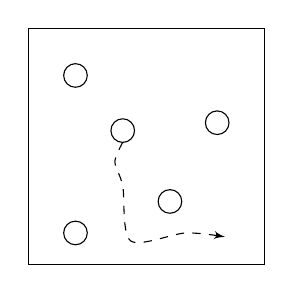
\begin{tikzpicture}
    \draw (0, 0) rectangle (3, 3);
    \draw (0.6, 0.4) circle [radius=0.15];
    \draw (1.8, 0.8) circle [radius=0.15];
    \draw (2.4, 1.8) circle [radius=0.15];
    \draw (0.6, 2.4) circle [radius=0.15];
    \draw (1.2, 1.7) circle [radius=0.15];
    \draw [-latex', dashed] plot [smooth] coordinates {(1.2, 1.55) (1.1, 1.3) (1.2, 1) (1.3, 0.3) (2, 0.4) (2.5, 0.35)};
  \end{tikzpicture}
\end{center}
In this regime, the colloid particles undergo Brownian motion, and we can ask how fast the particles move. It turns out The diffusivity constant is
\[
  D = \frac{k_B T}{6 \pi \eta_s a},
\]
where $\eta_s$ is the solvent viscosity. Thus, we can construct the timescale $\tau$ given by the time it takes to move through a distance of our own radius. In other words, we set $a^2 = D \tau$, and hence
\[
  \tau \sim \frac{a^3 \eta_s}{ k_B T}.
\]
When $\Phi > 0.55$, then the colloids fall into a crystal structure:
\begin{center}
  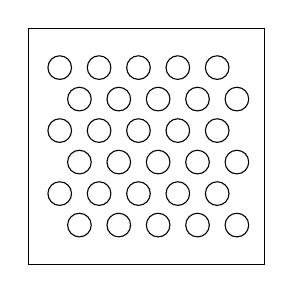
\begin{tikzpicture}
    \draw (-0.05, -0.1) rectangle +(3, 3);

    \draw (0.6, 0.4) circle [radius=0.15];
    \draw (1.1, 0.4) circle [radius=0.15];
    \draw (1.6, 0.4) circle [radius=0.15];
    \draw (2.1, 0.4) circle [radius=0.15];
    \draw (2.6, 0.4) circle [radius=0.15];

    \draw (0.35, 0.8) circle [radius=0.15];
    \draw (0.85, 0.8) circle [radius=0.15];
    \draw (1.35, 0.8) circle [radius=0.15];
    \draw (1.85, 0.8) circle [radius=0.15];
    \draw (2.35, 0.8) circle [radius=0.15];

    \draw (0.6, 1.2) circle [radius=0.15];
    \draw (1.1, 1.2) circle [radius=0.15];
    \draw (1.6, 1.2) circle [radius=0.15];
    \draw (2.1, 1.2) circle [radius=0.15];
    \draw (2.6, 1.2) circle [radius=0.15];

    \draw (0.35, 1.6) circle [radius=0.15];
    \draw (0.85, 1.6) circle [radius=0.15];
    \draw (1.35, 1.6) circle [radius=0.15];
    \draw (1.85, 1.6) circle [radius=0.15];
    \draw (2.35, 1.6) circle [radius=0.15];

    \draw (0.6, 2.0) circle [radius=0.15];
    \draw (1.1, 2.0) circle [radius=0.15];
    \draw (1.6, 2.0) circle [radius=0.15];
    \draw (2.1, 2.0) circle [radius=0.15];
    \draw (2.6, 2.0) circle [radius=0.15];

    \draw (0.35, 2.4) circle [radius=0.15];
    \draw (0.85, 2.4) circle [radius=0.15];
    \draw (1.35, 2.4) circle [radius=0.15];
    \draw (1.85, 2.4) circle [radius=0.15];
    \draw (2.35, 2.4) circle [radius=0.15];
  \end{tikzpicture}
\end{center}

Here the colloids don't necessarily touch, but there is still resistance to change in shape due to the entropy changes associated. We can find that the elasticity is given by
\[
  G \simeq k_B T \frac{N}{V}.
\]
In the small $\Phi$ case, the ``source'' of entropy is clear, given by the disorder in the position of the colloids. Here the entropy is given by the ``rattle room'' entropy.

In both cases, we see that the elasticity and time scales are given in terms of $k_B T$. If we ignore thermal fluctuations, then we have $G = 0$ and $\tau = \infty$, which is extremely boring, and more importantly, is not how the real world behaves!

\subsection{The general framework}
There are two parts to the study of soft condensed matters, confusingly and classically called \term{statics} and \term{dynamics}. The basic structure of the static part is going to look like this: we have some microscopic physics, but we don't want to track atoms and molecules. So we try to find some coarse-graining of the system. Thus, we come up with \emph{order parameter} fields, which we shall generically call $\psi(r)$. This goes into equilibrium statistical physics. To do this, we need to feed in symmetries and conservation laws. The output of this is some Boltzmann-distribution like probabilities $P[\psi(r)]$. In statistical physical field theory, $\psi$ might be our magnetization.

To do dynamics, we want to think of $\psi(r)$ as a function of space and time. The starting point is ``hydrodynamic'' PDEs of the form
\[
  \dot{\psi}(r, t) = \cdots,
\]
and the thing on the right hand side will depend on the type of substance we are talking about, and this is often informed by the static equilibrium statistical physics. The next step to realize is that even in dynamics, we cannot forget about thermal fluctuations. However, the PDE itself is deterministic. Thus, we have to promote these to stochastic PDEs, which are of the form
\[
  \dot{\psi}(r, t) = \cdots + \text{noise}.
\]
This is informed by the static probability given by the fluctuation dissipation theorem, which fixes the noise by requiring that it produces the right equilibrium statistics. If we have a stochastic equation like this, the basic thing we are trying to find out is the probability $\P[\psi(r, t)]$ of a certain evolution of a system, not only in space but also in time.

\begin{center}
  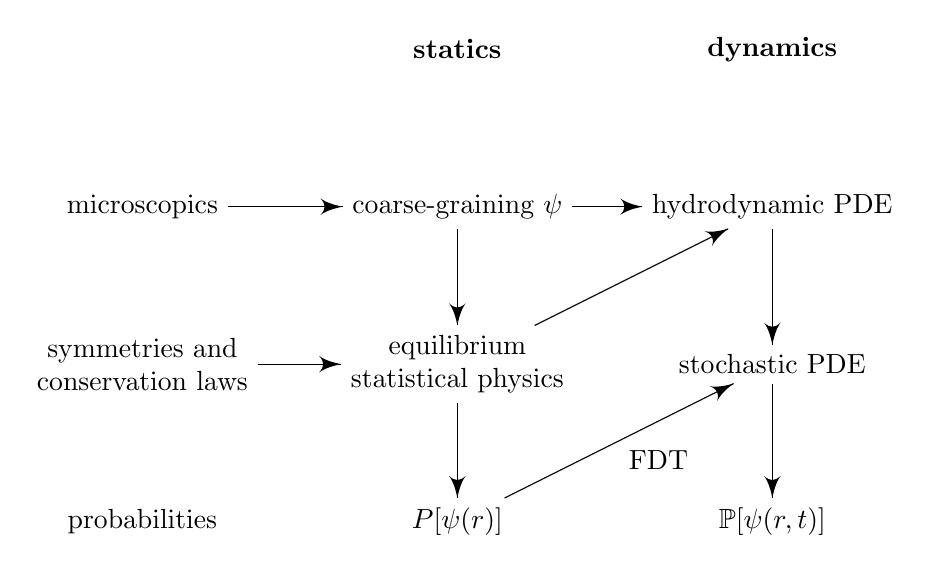
\begin{tikzpicture}[xscale=4, yscale=2]
    \node at (0, 0) {\textbf{statics}};
    \node at (1, 0) {\textbf{dynamics}};
    \node (mic) at (-1, -1) {microscopics};
    \node (coarse) at (0, -1) {coarse-graining $\psi$};
    \node (pde) at (1, -1) {hydrodynamic PDE};
    \node (sym) [align=center] at (-1, -2) {symmetries and\\ conservation laws};
    \node (equil) [align=center] at (0, -2) {equilibrium\\statistical physics};
    \node (stochastic) at (1, -2) {stochastic PDE};
    \node at (-1, -3) {probabilities};
    \node (p1) at (0, -3) {$P[\psi(r)]$};
    \node (p2) at (1, -3) {$\P[\psi(r, t)]$};

    \draw [->] (mic) -- (coarse);
    \draw [->] (sym) -- (equil);
    \draw [->] (coarse) -- (equil);
    \draw [->] (equil) -- (p1);
    \draw [->] (coarse) -- (pde);
    \draw [->] (pde) -- (stochastic);
    \draw [->] (equil) -- (pde);
    \draw [->] (p1) -- (stochastic) node [pos=0.5, anchor=north west] {FDT};
    \draw [->] (stochastic) -- (p2);
  \end{tikzpicture}
\end{center}
\begin{eg}
  $\psi(r, t)$ can consist of the density $\rho$ and velocity $\mathbf{v}$, and this describes a $1$-component isothermal fluid, e.g.\ water. The hydrodynamic PDE is exactly the fluid equations of motion.

  If we add a further composition function $\phi$, this describes a $2$-component fluid mixture. If we think about liquid crystals, then we need to add the molecular orientation. This actually requires a second-rank tensor $Q$, which describes a nematic liquid crystal.

  In the case of magnetism, we can add the magnetization $m$, but we will not do this in the course.
\end{eg}

\begin{eg}
  Consider isothermal, incompressible one-component fluid. The incompressibility condition is a simplification that lets us fix $\dot{\rho} = 0$. It follows that $\nabla \cdot \mathbf{v} = 0$. Then the equation in question is
  \[
    \rho (\dot{\mathbf{v}} + \mathbf{v} \cdot \nabla \mathbf{v}) = \eta \nabla^2 \mathbf{v} - \nabla p,
  \]
  the \term{Navier--Stokes equation}.

  We now promote this to a stochastic PDE. This is usually called the \term{Navier--Stokes--Landau--Lipschitz equation}, and is given by
  \[
    \rho (\dot{\mathbf{v}} + \mathbf{v} \cdot \nabla \mathbf{v}) = \eta \nabla^2 \mathbf{v} - \nabla p + \nabla \cdot \Sigma^N,
  \]
  The last term is thought of as a noise stress tensor on our fluid, and is conventionally treated as a Gaussian, and this is fixed by the fluctuation-dissipation theorem, and is given by
  \[
    \bra \Sigma_{ij}^N(r, t) \Sigma_{k \ell}^N (r', t')\ket = 2k_B T \eta (\delta_{i\ell} \delta_{jk} + \delta_{ik} \delta_{j\ell}) \delta(\mathbf{r} - \mathbf{r}') \delta(t - t').
  \]
\end{eg}

\section{Revision of equilibrium statistical physics}
\subsection{Thermodynamics}
The fastest route to getting the results we want is via Gibbs. We start with the notion of entropy
\[
  S = - k_B \sum_i p_i \log p_i,
\]
where $k_B$ is \term{Boltzmann's constant}, $i$ is a \term{microstate} --- a complete specification of the microscopics (e.g.\ the list of all particle coordinates and velocities) --- and $p_i$ is the probability of being in a certain microstate.

The axiom of Gibbs is that a system in thermal equilibrium maximizes $S$ subject to applicable constraints.
\begin{eg}
  In an isolated system, which has a fixed number $N$ of particles, and fixed energy $E$ and volume $V$. We now want to maximize $S$ subject to the only constraint
  \[
    \sum_i p_i = 1.
  \]
  Writing $\lambda$ for the Lagrange multiplier maintaining this constraint, we require
  \[
    \frac{\partial}{\partial p_i} \left(S - \lambda \sum_i p_i\right) = 0.
  \]
  So we find that
  \[
    -k_B \log p_i + 1 - \lambda = 0
  \]
  for all $i$. In particular, all $p_i$ must be equal. Note that the sum is restricted to fixed $N, E, V$. This is not the Boltzmann distribution, since we have completely isolated our system.
\end{eg}

\begin{eg}
  Consider a system of fixed contents ($N$) and volume $V$ in contact with a heat bath. So $E$ is no longer fixed, and fluctuates around some average $\bra E \ket = \bar{E}$. So we can apply Gibbs' principle again, where we now sum over all states of all $E$, with the restrictions
  \[
    \sum p_i E_i = \bar{E},\quad \sum p_i = 1.
  \]
  So our equation is
  \[
    \frac{\partial}{\partial p_i} \left(S - \lambda_I \sum p_i - \lambda_E \sum p_i E_i\right) = 0.
  \]
  Differentiating this with respect to $p_i$, we get
  \[
     -k_B (\log p_i + 1) - \lambda_I - \lambda_E E_i = 0.
  \]
  So it follows that
  \[
    p_i = \frac{1}{Z} e^{-\beta E_i},
  \]
  where $Z = \sum_i e^{-\beta E_i}$ and $\beta = \lambda_E/k_B$. This is the Boltzmann distribution.

  What is this mysterious $\beta$? Recall that the first law of thermodynamics says
  \[
    \d E = T\;\d S - P \;\d V + \mu \;\d N + \cdots.
  \]
  We can then read off
  \[
    \left.\frac{\partial S}{\partial E}\right|_{V, N, \ldots} = \frac{1}{T}.
  \]
  On the other hand, Gibb's principle says we should maximize $S - \lambda_E \bar{E}$, and so we have
  \[
    \frac{\partial S}{\partial E} = \lambda_E = \kappa_B \beta.
  \]
  So it follows that
  \[
    \beta = \frac{1}{k_B T}.
  \]
\end{eg}

Often, it is more useful to consider the free energy.
\begin{defi}[Helmholtz free energy]\index{Helmholtz free energy}
  The \emph{Helmholtz free energy} of a system at fixed temperature, volume and particle number is defined by
  \[
    F(T, V, N) = U - TS = \bar{E} - TS = - k_B T \log Z.
  \]
\end{defi}
This satisfies
\[
  \d F = -S \;\d T - P\;\d V + \mu\;\d N + \cdots,
\]
and is minimized at equilibrium for fixed $T, V, N$. The derivative of $F$ in an isothermal system tells us ``which way it moves''.

\subsection{Coarse Graining}
Usually, in statistical mechanics, we distinguish between two types of objects --- microstates, namely the exact configuration of the system, and macrostates, which are variables that describe the overall behaviour of the system, such that pressure and temperature. Here we would like to consider something in between.

For example, if we have a system of magnets as in the Ising model, we the microstate would be the magnetization at each site, and the macrostate would be the overall magnetization. A coarse-graining of this would be a function $m(\mathbf{r})$ of space that describes the ``average magnetization around $\mathbf{r}$''. There is no fixed prescription on how large an area we average over, and usually it does not matter much.

In general, the coarse-grained variable would be called $\psi$. We can define a coarse-grained partition function
\[
  Z[\psi(\mathbf{r})] = \sum_{i \in \psi} e^{-\beta E_i},
\]
where we sum over all states that coarse-grain to $\psi$. We can similarly define the energy and entropy by restricting to all such $\psi$, and get
\[
  F[\psi] = E[\psi] - T S[\psi].
\]
The probability of being in a state $\psi$ is then
\[
  \P[\psi] = \frac{e^{-\beta F[\psi]}}{Z_{TOT}},\quad Z_{TOT} = \int e^{-\beta F[\psi]} \;\D [\psi].
\]
What we have on the end is a \emph{functional integral}, where we integrate over all possible values of $\psi$. We shall go into details later. We then have
\[
  F_{TOT} = -k_B T \log Z_{TOT}.
\]
In theory, one can obtain $F[\psi]$ by explicitly doing a coarse graining of the macroscopic laws. However, what is more common is to take a phenomenological approach, which is to figure out a $F[\psi]$ empirically.

We first give an example of explicit coarse graining.
\begin{eg}
  Consider an ideal gas with $N$ particles.
\end{eg}
% something

Recall the free energy for a Landau--Ginzburg theory for a binary fluid, given by
\[
  \beta F = \int \Big(\underbrace{\frac{a}{2} \phi^2 + \frac{b}{4} \phi^4}_{f(\phi)} + \frac{K}{2} (\nabla \phi)^2\Big)\;\d x.
\]
We can do mean field theory with this. In our case, we look for a single $\phi(\mathbf{r})$ to minimize $F$ (i.e.\ to maximize $P \propto e^{-\beta F}$).

Since $\int \frac{K}{2} (\nabla \phi)^2\;\d x \geq 0$, we might guess that we should have a uniform $\phi$,
\[
  \phi(\mathbf{r}) = \bar{\phi}.
\]
Note that $\bar{\phi}$ is fixed by the constraint of the system, namely how much fluid of each type we have. Then
\[
  \frac{F}{V} = f(\bar{\phi}).
\]
We suppose $b$ is fixed, and $a = a(T)$. If $a > 0$, then the plot of $f$ looks like this:
\begin{center}
  \begin{tikzpicture}
     % insert picture, phase separation.
  \end{tikzpicture}
\end{center}
In the $a < 0$ case, we suppose the minima lie at $\phi_{1, 2} = \pm \phi_B$, where
\[
  \phi_B = \sqrt{\frac{-a}{b}}.
\]
Now if $\bar{\phi}$ lies between $\pm \phi_B$, then we have phase separation, where we have some bits with $\phi_0$ and others with $-\phi_0$, since
\[
  V_1 f(\phi_1) + V_2 f(\phi_2) < (V_1 + V_2) f(\bar{\phi}).
\]
We have the constraint
\begin{align*}
  V_1 \phi_1 + V_2 \phi_2 &= V \bar{\phi},\\
  V_1 + V_2 &= V.
\end{align*}
This phase separated state has a lower energy than the single phase version, at least if the gradient term is well-controlled.

We can now draw a mean-field phase diagram (with $b$ constant):
\begin{center}
  \begin{tikzpicture}
    \draw (-2, 3) node [above] {$a$} -- (-2, 0) node [below] {$-1$} -- (2, 0) node [below] {$1$} node [right] {$\bar \phi$} -- (2, 3);
    \node [left] at (-2, 2.5) {$a(T) = 0$};

    \draw [domain=2.5:0.2, samples=40] plot [smooth] ({sqrt (2.5 - \x)}, \x);
    \draw [domain=2.5:0.2, samples=40] plot [smooth] ({-sqrt (2.5 - \x)}, \x);

    \draw [dashed, domain=0.2:2.5] plot [smooth] ({sqrt ((2.5 - \x)/3)}, \x);
    \draw [dashed, domain=0.2:2.5] plot [smooth] ({-sqrt ((2.5 - \x)/3)}, \x);
    \draw (-2.05, 2.5) -- (-1.95, 2.5);
  \end{tikzpicture}
\end{center}
The inner curve is the spinodal instability, where we in fact have local instability, as opposed to global instability. This is given by the condition $f''(\bar{\phi}) < 0$, and this is given by
\[
  \phi_S = \sqrt{\frac{-a}{3b}}.
\]
What happens if we add a cubic term $\int \frac{c}{3} \phi(\mathbf{r})^3 \;\d \mathbf{r}$ to our $\beta F$? The motivation would be that the molecules might not be the same, and then there is no reason fundamentally between positive and negative values of the composition variables. We can also have a linear term, but as we have seen, it doesn't have an actual effect.

It turns out we can remove the $\phi(\mathbf{r})$ term by a linear shift of $\phi$ and $a$, which is a simple algebraic maneuver. So we have a shift of axes on the phase diagram.

The role of the gradient term $\int \frac{K}{2} (\nabla \phi)^2 \;\d \mathbf{r}$ captures at order $\nabla^{(2)}$ the non-locality of $E_{int}$,
\[
  E_{int} = \int \rho_i (\mathbf{r}) \rho_j(\mathbf{r}') U_{ij}(|\mathbf{r} - \mathbf{r}'|)\;\d \mathbf{r}\;\d \mathbf{r}',
\]
where $i, j \in A, B$. If we assume $\phi(\mathbf{r})$ is slowly varying on the scale of interactions, then we can Taylor expand this $E_{int}$ and obtain a $(\nabla \phi)^2$ term.

What does this do to our system? The parameter $K$ fixes the \term{interfacial tension},
\[
  \sigma = \left(\frac{-9 K a^3}{9 b^2}\right)^{1/2}.
\]
See questions 6, 7 on the example sheet.

\subsection{Landau--Ginzburg theory for nematic liquid crystals}
There are two basic ways of organizing rod-like molecules --- \term{isotropic} and \term{nematic}. In the first case, the rods are pointed in random directions, whereas in the nematic case, the rods all point in the same direction, i.e.\ there is a long range orientation order. However, there is no long-range positional order.

In the case of hard rods, we transition from isotropic to nematic when the density $\rho$ is increased.

The first and perhaps subtle point is that we have to pick an order parameter. Nematic molecules have a preferred \emph{axis}, but not a \emph{sense}, i.e.\ we can rotate our rod by $180^\circ$ and it still looks the same. Thus the orientation is represented by a ``headless vector'' $\nu$. Instead, it takes values in real projective space.

Given an arbitrary vector $A$, and $\mathbf{n}$ the direction of our rod, we can write down $(A \cdot \mathbf{n}) \mathbf{n}$ is the component of $\mathbf{A}$ along $\mathbf{n}$. While $A_i n_i n_j$ is a vector, $n_i n_j$ is a second-rank tensor, whose trace is $1$ (as $n$ is a unit vector). Crucially, if we flip the sign of all components of $n$, this does not change. If we have isotropic rods, then
\[
  \bra n_i n_j \ket = \frac{\delta_{ij}}{d},
\]
where $d$ is the number of dimensions. This allows us to introduce an order parameter
\[
  Q_{ij} (\mathbf{r}) = \bra n_i n_j\ket_{local} - \frac{1}{d} \delta_{ij}.
\]
Again, we need to pick a scale to do the coarse-graning. This is a traceless symmetric second-rank tensor, and vanishes in the isotropic phase, and non-zero in the nematic phase.

An interesting thing about this is that it is not conserved, i.e.\ $\int Q_{ij}(\mathbf{r})\;\d \mathbf{r}$ is not constant in time. This will have consequences for equilibrium statistical mechanics, but also the dynamics. So this is quite different from our previous binary fluid. We can follow the same procedure as we previously did, but it is going to be more complicated.

We have a free energy function. We start with the local part $f(Q)$, which is a scalar built on $Q$ via a Taylor series. So we need to find scalar invariants of $Q$.
\begin{enumerate}
  \item There is only one linear one, namely $Q_{ii} = \Tr(Q)$, but this vanishes.
  \item We can construct a quadratic term $Q_{ij} Q_{ji} = \Tr(Q^2)$, and this is in general non-zero.
  \item There is a cubic term $Q_{ij} Q_{jk} Q_{ki} = \Tr(Q^3)$, and is also in general non-zero.
  \item There are two possible quartic terms, namely $\Tr(Q^2)^2$ and $\Tr(Q^4)$.
\end{enumerate}
So we can write
\[
  f(Q) = a\Tr(Q^2) + c \Tr(Q^3) + b_1 \Tr(Q^2)^2 + b_2 \Tr(Q^4).
\]
This is the local part of the free energy up to fourth order in $Q$. We can go on, and in certain conditions we have to go on, but if these coefficients $b_i$ are sufficiently positive in some sense, we don't have to.

What can we say about the cubic term? Under what conditions do we expect $c$ to vanish? To understand this better, we fix $d = 3$, and consider the configuration
\[
  Q_{ij} =
  \begin{pmatrix}
    -\lambda/2 & 0 & 0\\
    0 & -\lambda/2 & 0\\
    0 & 0 & \lambda
  \end{pmatrix},\quad \lambda > 0.
\]
This arises if, for example, uniformly over the material, the rods are all likely to point in the $z$-direction. If $\lambda < 0$ instead, then the rods are all \emph{un}likely to point in the $z$-direction. There is absolutely no reason for these two states to have similar free energy, and the difference between the two is only captured in odd terms.

In the first example, we have
\begin{align*}
  f(Q) &= a \left(\frac{3}{2} \lambda^2\right) + c \left(\frac{3}{4} \lambda^3\right) + b_1\left(\frac{9}{4} \lambda^4\right) + b_2 \left(\frac{9}{8} \lambda^4\right)\\
  &= \bar{a} \lambda^2 + \bar{c} \lambda^3 + \bar{b}\lambda^4.
\end{align*}
This, we can think of this in a way similar to the binary fluid, where $\lambda$ is are sole order parameter. As a function of $\lambda$, where we vary $\bar{a}$ and fix $\bar{b}$ and $\bar{c} < 0$, we have
\begin{center}
  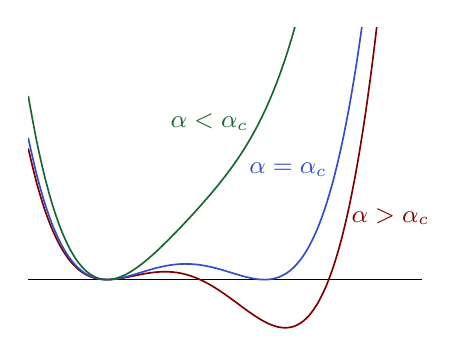
\begin{tikzpicture}[yscale=4]
    \draw (-1, 0) -- (4, 0);
    \clip (-1, -0.16) rectangle (4.3, 0.8);
    \draw [domain=-1:4, samples=50, mred, semithick] plot [smooth] (\x, {(\x)^2/6 - (\x)^3/5 + (\x)^4 / 20});
    \draw [domain=-1:4, samples=50, mblue, semithick] plot [smooth] (\x, {(\x)^2/5 - (\x)^3/5 + (\x)^4 / 20});
    \draw [domain=-1:4, samples=50, mgreen, semithick] plot [smooth] (\x, {(\x)^2/3 - (\x)^3/5 + (\x)^4 / 20});

    \node [mgreen] at (1.3, 0.5) {\small$\alpha < \alpha_c$};
    \node [mblue] at (2.3, 0.35) {\small$\alpha = \alpha_c$};
    \node [mred] at (3.6, 0.2) {\small$\alpha > \alpha_c$};
  \end{tikzpicture}
\end{center}
Here the cubic term gives a discontinuous transition. This is a first-order transition. If we had $\bar{c} > 0$ instead, then the minima are on the other side.

In general, cubic terms lead to discontinuous transitions.

We now move on to the gradient terms. We can have something of the form
\[
  F[Q] = \int \big(f(Q) + f_{\ell i}(\nabla_i Q_{kj})\big)\;\d \mathbf{r}.
\]
We do this to order $\nabla^{(2)}$ and $Q^{(2)}$. The only possible combinations are
\begin{align*}
  \kappa_1 \nabla_i \nabla_i Q_{j\ell} Q_{j\ell} &= \kappa_1 \nabla^2 \Tr(Q^2) \\
  \kappa_2 (\nabla_i Q_{im}) (\nabla_j Q_{jm}) &= \kappa_2(\nabla \cdot Q)^2\\
  \kappa_3 (\nabla_i Q_{jm}) (\nabla_j Q_{im}) &= \text{yuck}.
\end{align*}
Three linear combinations describe the following three things:
\begin{center}
  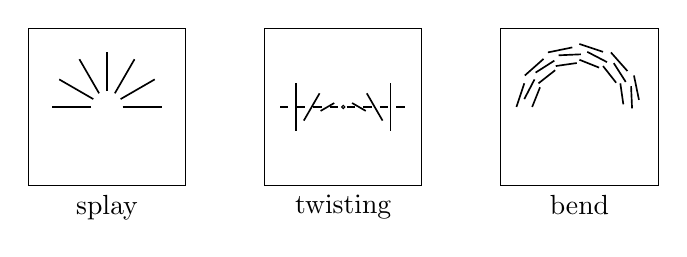
\begin{tikzpicture}
    \begin{scope}
      \draw (-1, -1) rectangle (1, 1);
      \node [below] at (0, -1) {splay};

      \draw [semithick] (0, 0.2) -- +(0, 0.5);
      \draw [semithick, rotate=30] (0, 0.2) -- +(0, 0.5);
      \draw [semithick, rotate=60] (0, 0.2) -- +(0, 0.5);
      \draw [semithick, rotate=90] (0, 0.2) -- +(0, 0.5);
      \draw [semithick, rotate=-30] (0, 0.2) -- +(0, 0.5);
      \draw [semithick, rotate=-60] (0, 0.2) -- +(0, 0.5);
      \draw [semithick, rotate=-90] (0, 0.2) -- +(0, 0.5);
    \end{scope}
    \begin{scope}[shift={(3, 0)}]
      \draw (-1, -1) rectangle (1, 1);
      \node [below] at (0, -1) {twisting};

      \draw [semithick] (-0.6, -0.3) -- +(0, 0.6);
      \draw [semithick] (0.6, -0.3) -- +(0, 0.6);

      \draw [semithick, rotate around={-30:(-0.4,0)}] (-0.4, -0.2) -- +(0, 0.4);
      \draw [semithick, rotate around={-60:(-0.2,0)}] (-0.2, -0.1) -- +(0, 0.2);

      \draw [semithick, rotate around={30:(0.4,0)}] (0.4, -0.2) -- +(0, 0.4);
      \draw [semithick, rotate around={60:(0.2,0)}] (0.2, -0.1) -- +(0, 0.2);

      \draw (0, 0) circle [radius=0.02];

      \draw [dashed, thin] (-0.8, 0) -- (0.8, 0);
    \end{scope}
    \begin{scope}[shift={(6, 0)}]
      \draw (-1, -1) rectangle (1, 1);
      \node [below] at (0, -1) {bend};

      \draw [semithick] (-0.8, 0) -- (-0.7, 0.3);
      \draw [semithick, rotate=-30] (-0.8, 0) -- (-0.7, 0.3);
      \draw [semithick, rotate=-60] (-0.8, 0) -- (-0.7, 0.3);
      \draw [semithick, rotate=-90] (-0.8, 0) -- (-0.7, 0.3);
      \draw [semithick, rotate=-120] (-0.8, 0) -- (-0.7, 0.3);
      \draw [semithick, rotate=-150] (-0.8, 0) -- (-0.7, 0.3);

      \draw [semithick] (-0.7, 0.1) -- (-0.57, 0.35);
      \draw [semithick, rotate=-30] (-0.7, 0.1) -- (-0.57, 0.35);
      \draw [semithick, rotate=-60] (-0.7, 0.1) -- (-0.57, 0.35);
      \draw [semithick, rotate=-90] (-0.7, 0.1) -- (-0.57, 0.35);
      \draw [semithick, rotate=-120] (-0.7, 0.1) -- (-0.57, 0.35);
      \draw [semithick, rotate=-150] (-0.7, 0.1) -- (-0.57, 0.35);

      \draw [semithick] (-0.6, 0) -- (-0.5, 0.25);
      \draw [semithick, rotate=-30] (-0.6, 0) -- (-0.5, 0.25);
      \draw [semithick, rotate=-60] (-0.6, 0) -- (-0.5, 0.25);
      \draw [semithick, rotate=-90] (-0.6, 0) -- (-0.5, 0.25);
      \draw [semithick, rotate=-120] (-0.6, 0) -- (-0.5, 0.25);
      \draw [semithick, rotate=-150] (-0.6, 0) -- (-0.5, 0.25);
    \end{scope}
  \end{tikzpicture}
\end{center}
Individually, we cannot see which $\kappa_i$ correspond to which modes, but they are given by some linear combinations.

The usual (simplest) choice is to set $\kappa_1 = \kappa_3 = 0$. If we make that choice, we find that there is a similar elastic cost to each of these deformations.

\section{Calculus review}
We first review some functional differentiation. Consider a scalar field $\varphi(\mathbf{r})$, and consider a functional
\[
  A[\phi] = \int L(\phi, \nabla \phi)\;\d \mathbf{r}.
\]
Consider a small change $\phi \mapsto \phi + \delta \phi(\mathbf{r})$, and we require $\delta \phi = 0$ on the boundary. Then
\begin{align*}
  A[\phi + \delta \phi] &= \int \left(L(\phi, \nabla \phi) + \delta \phi \frac{\partial L}{\partial \phi} + \nabla d \phi \cdot \frac{\partial L}{\partial \phi}\right)\;\d \mathbf{r}\\
  &= A[\phi] + \int \delta \phi \left(\frac{\partial L}{\partial \phi} + \nabla \cdot \frac{\partial L}{\partial \nabla \phi}\right)\;\d \mathbf{r},
\end{align*}
where we integrated by parts using the boundary condition. We then define\index{functional derivative}\index{$\frac{\delta A}{\delta \phi(\mathbf{r})}$}
\[
  \frac{\delta A}{\delta \phi(\mathbf{r})} = \frac{\partial L}{\partial \phi(\mathbf{r})} - \nabla \cdot \frac{\partial L}{\partial \nabla \phi}.
\]
\begin{eg}
  In classical mechanics, we replace $\mathbf{r}$ by the single variable $t$, and $\phi$ by position $x$. We then have
  \[
    A = \int L(x, \dot{x})\;\d t.
  \]
  Then we have
  \[
    \frac{\delta A}{\delta x(t)} = \frac{\partial L}{\partial x} - \frac{\d}{\d t} \left(\frac{\partial L}{\partial \dot{x}}\right),
  \]
  and in classical mechanics, we set this to zero.
\end{eg}

The example more relevant to us is perhaps Landau--Ginzburg theory:
\begin{eg}
  Consider a coarse-grained free energy
  \[
    F[\phi] = \int \left(\frac{a}{2} \phi^2 + \frac{b}{4} \phi^4 + \frac{K}{2} (\nabla \phi)^2 \right)\;\d \mathbf{r}.
  \]
  Then
  \[
    \frac{\delta F}{\delta \phi(\mathbf{r})} = a \phi + b \phi^3 - K \nabla^2 \phi.
  \]
  In mean field theory, we set this to zero, since by definition, we are choosing a single $\phi(\mathbf{r})$ that minimizes $F$. In the example sheet, we solve this to get
  \[
    \phi(x) = \phi_B \tanh \left(\frac{x - x_0}{\xi_0}\right).
  \]
\end{eg}

For a general $F[\psi]$, we can think of the functional derivative $\frac{\delta F}{\delta \psi(\mathbf{r})}$ as a ``generalized force'', and it tells the system which way to move in order to reduce the free energy. Recall that
\[
  \d F = - S \;\d T - p \;\d V + \mu \;\d N + \mathbf{h} \cdot \d \mathbf{M} + \cdots.
\]
We can then think of
\[
  \delta F = \int \frac{\delta F}{\delta \psi(\mathbf{r})} \delta \psi(\mathbf{r})\;\d r.
\]
as an additional term, and we can think of $\frac{\delta F}{\delta \psi(\mathbf{r})}$ as the intensive variable, while $\delta \psi(\mathbf{r})$ is the extensive variable. If $\psi$ is the particle density, for example, then we can think of these as the $\mu$ and $N$ respectively. If it is the magnetization, then these would be like $\mathbf{h}$ and $\mathbf{M}$.

Note that for $\psi$ a conserved scalar density $(\rho, \phi)$, the quantity
\[
  \mu(\mathbf{r}) = \frac{\delta F}{\delta \phi(\mathbf{r})}
\]
is called the \term{chemical potential}.

On the other hand, if $\psi$ is not conserved, e.g.\ the $Q$ we had before, then
\[
  H_{ij} = \frac{\delta F}{\delta Q_{ij}}
\]
is called the \emph{molecular field}.

In the case where $\phi$ is conserved, we have the conservation law
\[
  \dot{\phi} = - \nabla \cdot J.
\]
This $J$ is then given by an equation of the form
\[
  J \propto -D \nabla \mu,
\]
where $D$ is the diffusivity.

The non-conserved case is simpler. We have
\[
  \dot{Q} = - \Gamma H.
\]
This is local relaxation.

Let us go back to the scalar field $\phi(\mathbf{r})$. Consider a small displacement
\[
  \mathbf{r} \mapsto \mathbf{r} + \mathbf{u}(\mathbf{r}).
\]
We take this to be incompressible, so that $\nabla \cdot \mathbf{u} = 0$. Then
\[
  \phi \mapsto \phi' = \phi'(\mathbf{r}) = \phi(\mathbf{r} - \mathbf{u}).
\]
Then
\[
  \delta \phi(\mathbf{r}) = \phi'(\mathbf{r}) - \phi(\mathbf{r}) = - \mathbf{u} \cdot \nabla \phi(\mathbf{r}) + O(u^2).
\]
Then
\begin{align*}
  \delta F &= \int \delta \phi \frac{\delta F}{\delta \phi}\;\d \mathbf{r} \\
  &= -\int \mu \mathbf{u} \cdot \nabla \phi \;\d \mathbf{r}\\
  &= \int \phi \nabla \cdot (\mu \mathbf{u})\;\d \mathbf{r}\\
  &= \int (\phi \nabla \mu)\cdot \mathbf{u}\;\d \mathbf{r}\\
  &= \int (\phi \nabla_j \mu)u_j\;\d \mathbf{r}.
\end{align*}
using incompressibility.

We can think of the free energy change as the work done by stress,
\[
  \delta F = \int \sigma_{ij}(\mathbf{r}) \varepsilon_{ij}(\mathbf{r})\;\d \mathbf{r},
\]
where $\varepsilon_{ij} = \nabla_i u_j$ is the strain tensor, and $\sigma_{ij}$ is the stress tensor. So we can write this as
\[
  \delta F = \int \sigma_{ij} \nabla_i u_j\;\d \mathbf{r} = - \int (\nabla_i \sigma_{ij}) u_j\;\d \mathbf{r}.
\]
So we can identify
\[
  \nabla_i \sigma_{ij} = -\phi \nabla_j \mu.
\]
So $\mu$ also contains the ``mechanical information''.

\subsection{Functional integrals}
Given a coarse-grained $\psi$, we have can define the total partition function
\[
  e^{-\beta F_{TOT}} = Z_{TOT} = \int e^{-\beta F[\psi]} \;\D [\psi],
\]
where $\D [\psi]$ is the ``sum over all field configurations''. To make sense of this, the simplest implementation is to move to Fourier space, and write
\[
  F[\psi] = F\{\psi_\mathbf{q}\}.
\]
with each $\psi_\mathbf{q}$ representing a Fourier mode, defined by
\[
  \psi_\mathbf{q} = \frac{1}{\sqrt{V}} \int \psi(\mathbf{r}) e^{-i\mathbf{q}\cdot \mathbf{r}}\;\d \mathbf{r},
\]
where $V = L^q$ is our region with periodic boundary conditions. This normalization is chosen so that
\[
  \int |\psi|^2 \;\d \mathbf{r} = \sum_{\mathbf{q} } |\psi_\mathbf{q}|^2.
\]
This is known as \term{Parseval's theorem}.

There is now a countable list of complex variables $\psi_\mathbf{q}$. We can then define
\[
  \D [\psi] = \prod_{\mathbf{q}} \;\d \psi_\mathbf{q}.
\]
We will want to set a $q_{max}$ to make the product finite, which is set by molecular physics or coarse graining. We will mostly focus on things that are mostly independent of this.

The protocol is to keep $V < \infty$ until we are done, and then take the thermodynamic limit $V \to \infty$ if we want. In this limit, the sum over $\mathbf{q}$ becomes an integral, and it is harder to make sense of $\D[\psi]$.

In practice, there is only one integral like this that can be done. Everything we do is a deformation of the same thing, expanded and understood using perturbation. The case where we can do is when $\beta F$ is a quadratic form. Suppose
\[
  \beta F = \frac{1}{2} \int \phi(\mathbf{r}) G(\mathbf{r} - \mathbf{r}') \phi(\mathbf{r}')\;\d \mathbf{r}\;\d \mathbf{r}'. - \int h(\mathbf{r}) \phi(\mathbf{r})\;\d \mathbf{r}.
\]
This is a generalization of what we want, where the gradient terms are essentially localizations of the difference between evaluations at two points. Then
\[
  \beta F[\psi_\mathbf{q}] = \frac{1}{2} \sum_q G(\mathbf{q}) \phi_\mathbf{q} \phi_{-\mathbf{q}} - \sum_\mathbf{q} h_\mathbf{q} \phi_\mathbf{q}.
\]
Note that $\phi$ is real, which is equivalent to $\phi_\mathbf{q} = - \phi_\mathbf{q}^*$. So we only integrate over a half space, and we denote this by writing $\prod_\mathbf{q}^+$ instead.
\begin{eg}
  We take Landau--Ginzburg theory
  \[
    \beta F[\phi] = \int \left\{\xi \phi^2 + \frac{b}{4} \phi^4 - h \phi + \frac{\kappa}{2} (\nabla \phi)^2 + \frac{\gamma}{2} (\nabla^2 \phi)^2\right\}\;\d \mathbf{r}
  \]
  and then we set $b = 0$ since this is the scenario we know how to deal with. We will later see how we can put it back. The $\gamma$ term is necessary because we will be interested in the case where $\kappa$ is negative.

  We can now take the Fourier transform to get
  \begin{align*}
    \beta F \{\phi_\mathbf{q}\} &= \frac{1}{2} \sum_\mathbf{q} (a + \kappa q^2 + \gamma q^4) \phi_\mathbf{q} \phi_{-\mathbf{q}} - \sum_\mathbf{q} h_\mathbf{q} \phi_\mathbf{q}.\\
    &= \sum_\mathbf{q}^+ (a + \kappa q^2 + \gamma q^4) \phi_\mathbf{q} \phi_{-\mathbf{q}} - \sum_\mathbf{q} h_\mathbf{q} \phi_\mathbf{q}.
  \end{align*}
  So our $G(\mathbf{q})$ is given by
  \[
    G(\mathbf{q}) = a + k q^2 + \gamma q^4,
  \]
  which we can think of a Taylor expansion of something more fancy. This is of the stated form. For $h = 0$, we have
  \begin{align*}
    Z_{TOT} &= \int \left[ \prod_{\mathbf{q}}^+ \;\d \phi_\mathbf{q}\right] e^{-\beta F\{\phi_\mathbf{q}\}}\\
    &= \prod_\mathbf{q}{\vphantom{\prod}}^+ \int \d \phi_\mathbf{q} e^{-|\phi_\mathbf{q}|^2 G(q)}
  \end{align*}
  Consider a single integral
  \[
    \int \d \phi_\mathbf{q} e^{-|\phi_\mathbf{q}|^2 G(q)} = \int \rho \;\d \rho \;\d \theta e^{-G(q) \rho^2} = \frac{\pi}{G(q)}.
  \]
  where $\phi_\mathbf{q} = \rho e^{i\theta}$.

  So we find that
  \[
    Z_{TOT} = \prod_\mathbf{q}{\vphantom{\prod}}^+ \frac{\pi}{G(q)},
  \]
  and so
  \[
    \beta F_T = -\log Z_T = \sum_\mathbf{q}{\vphantom{\sum}}^+ \log \frac{G(q)}{\pi}.
  \]
  We now take large $V$ limit, and replace the sum of the integral. Then we get
  \[
    \beta F_T = \frac{1}{2} \frac{V}{(2\pi)^d} \int^{q_{max}} \;\d \mathbf{q} \log \frac{G(q)}{\pi}.
  \]
  For the $h \not= 0$ case, we complete the square and apply this result.
\end{eg}

\begin{eg}
  Consider the ``\term{structure factor}''
  \[
    S(\mathbf{k}) = \bra \phi_\mathbf{k} \phi_{-\mathbf{k}}\ket = \frac{1}{Z_T} \int \phi_\mathbf{k} \phi_{-\mathbf{k}} e^{-\sum_\mathbf{q}^+ \phi_\mathbf{q} \phi_{-\mathbf{q}} G(q)} \prod_q{}^+ \;\d \phi_\mathbf{q}.
  \]
  We see that this is equal to
  \[
    \frac{1}{Z_T} \frac{\partial Z_T}{\partial G(\mathbf{k})} = - \frac{\partial \log Z_T}{\partial G(\mathbf{k})} = \frac{1}{G(k)}.
  \]
  Note that we could also have done this explicitly using the product expansion.

  This $S(k)$ is measured in scattering experiments. For small $k$ and $\kappa > 0$, we have
  \[
    S(q) = \frac{1}{a + \kappa k^2 + \gamma k^4} \approx \frac{a^{-1}}{1 + k^2 \xi^2},
  \]
  where $\xi$ is the \term{correlation length}, given by
  \[
    \xi = \sqrt{\frac{\kappa}{a}}.
  \]
  We can return to real space by
  \begin{align*}
    \bra \phi^2(\mathbf{r})\ket &= \frac{1}{V} \left\bra \int |\phi(\mathbf{r})|^2 \;\d \mathbf{r}\right\ket \\
    &= \frac{1}{V} \sum_q \bra \phi_\mathbf{q}|^2\ket\\
    &= \frac{1}{(2\pi)^d} \int^{q_{max}} \frac{\d \mathbf{q}}{a + \kappa q^2 + \gamma q^4}.
  \end{align*}
\end{eg}

For now, we restore the $\phi^4$ term in Landau--Ginzburg theory. We know that mean field theory with Gaussian fluctuations fail near the critical point. This is the kickoff for renormalization group theory, which is not the content of this course. Between mean field theory and renormalization group is another level of approximation, which is a variational method. % Landau Ginzburg fails for $\bar{\phi}$ near $\pm 1$ as well.

In condensed matter physics, this is known as \term{Hartree theory}, and in QFT it is known as ``\term{1-loop self consistency}''. In this theory, large Gaussian fluctuations are okay, and this occurs in case such as smectic liquid crystals.

To understand this, we wlog assume $\beta = 1$. Then we have
\[
  e^{-F_{TOT}} = \int e^{-F[\phi]}\;\D [\phi].
\]
We now make a notation change, where we write $F_{TOT}$ as $F$, and we now write $F[\phi]$ as $H[\phi]$ instead, called \term{the effective Hamiltonian}. In this notation, we write
\[
  e^{-F} = \int e^{-H[\phi]} \;\D [\phi].
\]
We introduce a \term{trial Hamiltonian} $H_0[\phi]$. Then we can look at
\[
  e^{-F_0} = \int e^{-H_0[\phi]} \;\D [\phi].
\]
Hence we have
\begin{align*}
  e^{-F} &= \frac{e^{-F_0}}{\int e^{-H_0}\;\D [\phi]} \int e^{-H_0} e^{-(H - H_0)}\;\D [\phi] \\
  &= e^{-F_0} \bra e^{-(H - H_0)} \ket_0,
\end{align*}
where we are taking the average over the trial distribution. So far, this is exact, but this is going to be the basis for approximation.

If we just take the logarithm, we find
\[
  F = F_0 - \log \bra e^{-(H - H_0)}\ket_0.
\]
Observe that the function $\log$ is concave. In other words,
\[
  \log (\alpha A + (1 - \alpha) B) \geq \alpha \log A + (1 - \alpha) \log B.
\]
Hence by Jensen's inequality, we have
\[
  \log \bra Y \ket_0 \geq \bra \log Y \ket_0.
\]
Applying this to our situation gives us an inequality
\[
  F \leq F_0 - \bra H_0 - H\ket_0 = F_0 - \bra H_0\ket_0 + \bra H\ket_0 = S_0 + \bra H\ket_0.
\]
This is the \term{Feynman--Bogoliubov inequality}.

To use this, we have to choose the trial distribution $H_0$ simple enough to actually do calculations (i.e.\ Gaussian), but include variational parameters in $H_0$. We then minimize the quantity $F_0 - \bra H_0\ket + \bra H\ket_0$ over our variational parameters, and this gives us a least upper bound on $F$, which we take to be our best estimate of $F$.

We use this to talk about the isotropic to smectic transition. Examples include soap molecules, which look like
\begin{center}
  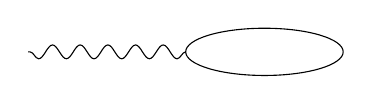
\begin{tikzpicture}
    \draw (0, 0) ellipse (1 and 0.3);
    \draw [decorate, decoration=snake] (-1, 0) -- (-3, 0);
  \end{tikzpicture}
\end{center}
where the tail $A$ hates water and the head $B$ likes water. There are some possible variations on these. For example, we can have two ``heads'' that like to be away from each other, or we can have two long tails covalently joined together, behaving similarly.

As we did with the binary fluid, we shall take the symmetric case for simplicity, so $U_{AA} = U_{BB} \not= U_{AB}$. A simple configuration might look like

\begin{center}
  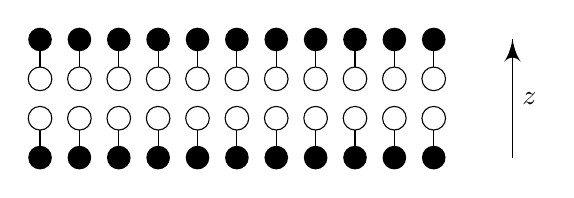
\begin{tikzpicture}[scale=0.5]
    \foreach \x in {0,...,10} {
      \begin{scope}[shift={(\x, 0)}]
        \fill circle [radius=0.3];
        \draw (0, -1) circle [radius=0.3];
        \draw (0, -2) circle [radius=0.3];
        \fill (0, -3) circle [radius=0.3];
        \draw (0, -0.3) -- (0, -0.7);
        \draw (0, -2.3) -- (0, -2.7);
      \end{scope}
   }

   \draw [->] (12, -3) -- (12, 0) node [pos=0.5, right] {$z$};
  \end{tikzpicture}
\end{center}
So we have a $1d$ lattice in the vertical direction with period $\lambda$, and is a fluid in the two remaining directions. This is known as a \term{smectic liquid crystal}, and is also known as the \term{lamellar phase}. This is an example of \term{microphase separation}.

We return to the Landau--Ginzburg model again. Back to our old notation, we have
\[
  \beta F = \int \left(\frac{a}{2} \phi^2 + \frac{b}{4} \phi^4 + \frac{\kappa}{2} (\nabla \phi)^2 + \frac{\gamma}{2} (\nabla^2 \phi)^2\right)\;\d \mathbf{r}.
\]
If we write this in Fourier space, then we get
\[
  \beta F = \frac{1}{2} \sum_{\mathbf{q}} (a + \kappa q^2 + \gamma q^4) \phi_{\mathbf{q}} \phi_{-\mathbf{q}} + \frac{b}{4V} \sum_{\mathbf{q}_1, \mathbf{q}_2, \mathbf{q}_3} \phi_{\mathbf{q}_1} \phi_{\mathbf{q}_2} \phi_{\mathbf{q}_3} \phi_{-(\mathbf{q}_1 + \mathbf{q}_2 + \mathbf{q}_3)}.
\]
For the iso-smectic transition, we choose $\kappa < 0, \gamma > 0$.

Without $b$, we have a Gaussian model, and
\[
  G(q) = a + \kappa q^2 + \gamma q^4.
\]
For different $a$, this looks like
\begin{center}
  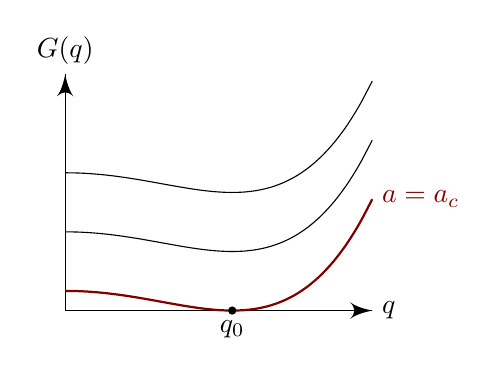
\begin{tikzpicture}[xscale=3]
    \draw [->] (0, 0) -- (1.3, 0) node [right] {$q$};
    \draw [->] (0 ,0) -- (0, 3) node [above] {$G(q)$};

    \draw [domain=0:1.3] plot [smooth] (\x, {1 - \x^2 + \x^4});
    \draw [domain=0:1.3, thick, mred] plot [smooth] (\x, {0.25 - \x^2 + \x^4});
    \draw [domain=0:1.3] plot [smooth] (\x, {1.75 - \x^2 + \x^4});
    \node [right, mred] at (1.3, 1.4161) {$a = a_c$};

    \node [circ] at (0.707, 0) {};
    \node [below] at (0.707, 0) {$q_0$};
  \end{tikzpicture}
\end{center}

Thus, as $a$ decreases $S(q) = \bar |\phi_\mathbf{q}|^2 = \frac{1}{G(q)}$ is going to blow up at some finite
\[
  q = q_0 = \sqrt{\frac{-\kappa}{2\gamma}},\quad a_c = \frac{\kappa^2}{4 \gamma}.
\]
If we think about this, then this is saying we really want to always stay at the fixed $q_0$, and this gives us an ordered phase.

Just for convenience now, we are going to expand $G$ about $q = q_0$ and $a = a_c$. Then we have
\[
  G(q) = \tau + \alpha(q - q_0)^2,
\]
where
\[
  \tau = a - a_0,\quad \alpha = \frac{1}{2} G''(q_0) = - 2\kappa.
\]
We now have to put back the quartic term. We first do this with mean field theory, and then later return to the variational method.

In mean field theory, it is easier to work in real space. In mean field theory, we look for a single field configuration that minimizes $F$. We can put
\[
  \phi = A \cos q_0 z,
\]
which is smectic along $z$. The direction of $z$ is arbitrary, and we have a spontaneously broken rotational symmetry. We can then evaluate
\[
  \frac{\beta F}{V} = \beta \overline{F[\phi]},
\]
where the bar means we average over one period of the periodic structure. We then compute this to be
\[
  \beta \overline{F[\phi]} = \frac{a}{2} \overline{\phi^2} + \frac{\kappa}{2} \overline{(\nabla \phi)^2} + \frac{\gamma}{2} \overline{(\nabla^2 \phi)^2} + \frac{b}{4} \overline{\phi^4}
\]
We have
\[
  \overline{\phi^2} = \frac{1}{2} A^2,\quad \overline{(\nabla \phi)^2} = \frac{1}{2} A^2 q_0^2,\quad \overline{(\nabla^2 \phi)^2} \frac{1}{2} A^2 q_0^4,\quad \overline{\phi^4} = \frac{3}{8} A^4.
\]
We have
\[
  \frac{\beta F}{V} = \frac{1}{4} \left[aA^2 + \kappa A^2 q_0^2 + \gamma A^2 q_0^4 + \frac{3b}{8} A^4\right] = \frac{1}{4} \left[ A^2 \underbrace{(a - a_c)}_\tau + \frac{3b}{8} A^4\right].
\]
Note that $q_0$ is fixed by the system as we originally had, while $A$ is the amplitude of the fluctuation which we get to choose.
\begin{center}
  \begin{tikzpicture}[xscale=1.5];
    \draw [->] (-2, 0) -- (2, 0) node [right] {$A$};
    \draw [->] (0, -1) -- (0, 3.5) node [above] {$\beta F/V$};
    \draw [domain=-2:2, mblue, semithick] plot (\x, {(\x)^2/4 + (\x)^4/8});
    \draw [domain=-2:2, mred, semithick] plot (\x, {-(\x)^2/3 + (\x)^4/8});

    \node [right, mblue] at (2, 3) {$\tau > 0$};
    \node [right, mred] at (2, 0.667) {$\tau < 0$};
    \node [left, white] at (-2, 3) {$\tau > 0$};
    \node [left, white] at (-2, 0.667) {$\tau < 0$};
  \end{tikzpicture}
\end{center}
To find the best $\phi$, we need to consider the different possibilities of $\tau$. If $\tau > 0$, then we should pick $A = 0$. Otherwise, we should pick $A \not= 0$, and we have a continuous transition to layered state.

\begin{center}
  \begin{tikzpicture}
    \draw [->] (0, 0) -- (4, 0) node [right] {$a$};
    \draw [->] (0, 0) -- (0, 3);

    \draw [mblue, semithick] (3.9, 0) -- (2, 0);
    \draw [domain=0:2, mblue, semithick, samples=30] plot [smooth] (\x, {sqrt(2 - \x)});
  \end{tikzpicture}
\end{center}
We now consider the variational theory, with Gaussian fluctuations. In the notation we were using previously, we have
\[
  H = \sum_\mathbf{q} {}^+ \phi_\mathbf{q} \phi_{-\mathbf{q}} G(q) + \frac{b}{4V} \sum_\mathbf{q} \phi_{\mathbf{q}_1} \phi_{\mathbf{q}_2} \phi_{\mathbf{q}_3} \phi_{-(\mathbf{q}_1 + \mathbf{q}_2 + \mathbf{q}_3)}.
\]
Our trial $H_0$ is
\[
  H_0 = \sum_\mathbf{q} \phi_\mathbf{q} \phi_{-\mathbf{q}} J(q).
\]
Since this is a Gaussian model, we know that
\[
  F_0 = \sum_{\mathbf{q}} {}^+ \log \frac{J(q)}{\pi}.
\]
To use our inequality, we need to evaluate our other two bits. We have
\[
  \bra H_0\ket_0 = \sum_{\mathbf{q}}{}^+ \bra \phi_\mathbf{q} \phi_{-\mathbf{q}}\ket_0 J(q).
\]
We already calculated
\[
  \bra \phi_{\mathbf{q}} \phi_{-\mathbf{q}} \ket_0 = \frac{1}{J(q)}.
\]
Thus, we have
\[
  \bra H_0 \ket_0 = \sum_{\mathbf{q}} {}^+ 1.
\]
Here it is clear that we must impose a cutoff on $\mathbf{q}$. We can think of this $1$ as the equipartition theorem.

We can also compute
\[
  \bra H\ket_0 = \sum_\mathbf{q} {}^+ \frac{1}{J(q)} G(q) + \frac{b}{4V} \underbrace{\sum_{\mathbf{q}_1, \mathbf{q}_2, \mathbf{q}_3}\bra \phi_{\mathbf{q}_1} \phi_{\mathbf{q}_2} \phi_{\mathbf{q}_3} \phi_{-(\mathbf{q}_1 \mathbf{q}_2 \mathbf{q}_3)}\ket_0}.
\]
In the Gaussian model, each $\phi_\mathbf{q}$ is a zero mean Gaussian random variables, which have certain nice properties. This is known as \term{Wick's theorem}, which tells us
\[
  \bra abcd \ket_0 = \bra ab\ket_0 \bra cd\ket_0 + \bra ac\ket_0 \bra bd\ket_0 + \bra ad\ket_0 \bra bc\ket_0.
\]
We also have
\[
  \bra \phi_{\mathbf{q}_1} \phi_{\mathbf{q}_0}\ket = \bra |\phi_\mathbf{q}|^2 \ket_0 \delta_{\mathbf{q}_1, - \mathbf{q}_2}.
\]
This gives the result
\[
  U = 3 \left[\sum_\mathbf{q} \bra |\phi_\mathbf{q}|^2\ket_0\right]^2 = 12 \left[\sum_\mathbf{q} {}^+ \frac{1}{J(q)}\right]^2.
\]
Thus, we have
\[
  \bra H_0\ket_0 = \sum_{\mathbf{q}} {}^+ \frac{G(q)}{J(q)} + \frac{3b}{V} \left(\sum_\mathbf{q} {}^+ \frac{1}{J(q)}\right)^2.
\]
We can then compute
\[
  \tilde{F} = \sum_{\mathbf{q}} {}^+ \left(\log \frac{J(q)}{\pi} - 1 + \frac{G(q)}{J(q)}\right) + \frac{3b}{V}\left(\sum_\mathbf{q} {}^+ \frac{1}{J(q)}\right)^2.
\]
We minimize over $J(q)$ by solving
\[
  \frac{\partial \tilde{F}}{\partial J(q)} = 0
\]
for all $\mathbf{q}$. Differentiating, we obtain
\[
  \frac{1}{J(q)} - \frac{G(q)}{J(q)^2} - \frac{6b}{V J(q)^2} \sum_{\mathbf{q}'} {}^+ \frac{1}{J(q')} = 0.
\]
Multiplying through by $J^2$, we get
\[
  J(q) = G(q) + \frac{6b}{V} \sum_{\mathbf{q}'} {}^+ \frac{1}{J(q')}.
\]
For large $V$, we can replace the sum by an integral, and we have
\[
  J(q) = G(q) + \frac{3b}{(2\pi)^d} \int \frac{\d \mathbf{q}'}{J(\mathbf{q}')}.
\]
It is very important that the second term is not a function of $\mathbf{q}$. So what we have got is that $J(q)$ is a constant plus $G(q)$. Informally, there is another way of viewing these types of calculations. This is a self-consistent treatment of the quartic. This is equivalent to making the following ad hoc approximation inside the Landau--Ginzburg theory.
\[
  \int \left\{ \frac{a}{2} \phi^2 + \frac{b}{4} \phi^4\right\} \;\d \mathbf{r} \mapsto  \int \left\{ \frac{a}{2} \phi^2 + \frac{3b}{2} \bra \phi^2 \ket \phi^2\right\}\;\d \mathbf{r}'
\]
While $\bar \phi^2\ket = \bra \phi(\mathbf{r})^2\ket$ is the average over all ensembles at a fixed point $\mathbf{r}$, it is equal to what we get by averaging over all points, so
\[
  \bra \phi(\mathbf{r})^2\ket = \frac{1}{V} \int \bra \phi(\mathbf{r})^2\ket \;\d \mathbf{r} = \frac{1}{V} \sum_q \bra |\phi_\mathbf{q}|^2 \ket = \frac{1}{V} \sum_{\mathbf{q}} \frac{1}{J(\mathbf{q})}.
\]
The only perhaps sightly stricky part if we were to just do this ad hoc is the factor of $\frac{3b}{2}$.

In our original omdel, we have
\[
  G(q) = \tau + \alpha(q - q_0)^2.
\]
We then have
\[
  J(q) = \bar{\tau} + \alpha (q - q_0)^2,
\]
where
\[
  \bar{\tau} = \tau + \frac{3b}{(2\pi)^d} \int \frac{\d^d \mathbf{q}}{\bar{\tau} + \alpha(q - q_0)^2}.
\]
We now have to solve this for $\bar{\tau}$. Close to the critical point, $\bar{\tau}$ is small. When $d = 3$, we have
\[
  \frac{3b}{(2\pi)^d} \int \frac{\d^d q}{\bar{\tau} + \alpha (q - q_0)^2} \approx q_0^2 \frac{3b}{2\pi^2} \int_0^\infty \frac{\d q}{\bar{\tau} + \alpha (q - q_0)^2},
\]
using the fact that the integral is largely peaked at $q = q_0$ (we would normally have a $q^2$ inside the integral rather than a $q_0^2$ outside). % this needs a cutoff to make sense

By non-dimensionalizing, we can write
\[
  \bar{\tau} = \tau + \frac{sb}{\sqrt{\bar{\tau}}},\quad s = \frac{3q_0^2}{2\pi^2} \frac{1}{\sqrt{\alpha}} \int_0^\infty \frac{\d y}{1 + y^2} \sim \frac{q_0^2}{\sqrt{\alpha}}. % mass renormalization
\]
Note that $\bar{\tau}$ can never approach zero! This means we can never have a continuous transition. At small $\bar{\tau}$, we have large fluctuations, but self-limiting arises on shell $q = q_0$. We have many modes contributing to the Gaussian approximation. The quantity
\[
  \bra |\phi_\mathbf{q}|^2 \ket = s(q) = \frac{1}{\bar{\tau} + \alpha(q - q_0)^2}
\]
does not diverge at $q = q_0$. So the isotropic-smectic transition must be discontinuous.

The idea is that fluctuations induces first-order transitions.

Consider fluctuations about an ordered state, $\phi = \phi_0 + \delta \phi$, and we set
\[
  \phi_0 = A \cos q_0 z.
\]
A formal approach to this would be to set
\[
  H_0 = \sum_{\mathbf{q}} {}^+ J(q) + hA,
\]
where we think of $h$ as a Lagrangian multiplier for $A$. We minimize $\tilde{F}(A)$ over $J(q)$. then $\tilde{F}(A)$ replaces
\[
  F_{MFT}(A) = \frac{V}{4} \left[\tau A^2 + \frac{3b}{8} A^4\right].
\]
This is actually quite messy, so let us do a heuristic version instead. For $A = 0$, we had
\[
  \tau = \bar{\tau} + 3b \bra \overline{\phi(\mathbf{r})^2}\ket.
\]
We can apply this for finite $A$. Then the quartic piece, where the $\phi^4$ term now has an extra contribution. So we have
\[
  \bar{\tau} = \tau + \frac{sb}{\sqrt{\bar{\tau}}} + \frac{3b A^2}{2}.
\]
If $A$ is small enough, then fluctuations dominate, and the transition is first order. For large $A$, the fluctuation terms are irrelevant, and mean field theory is good.

Recall that for mean field theory, our function $F$ looked like
\begin{center}
  \begin{tikzpicture}[xscale=1.5];
    \draw [->] (-2, 0) -- (2, 0) node [right] {$A$};
    \draw [->] (0, -1) -- (0, 3.5) node [above] {$F_{MFT}$};
    \draw [domain=-2:2, mblue, semithick] plot (\x, {(\x)^2/4 + (\x)^4/8});
    \draw [domain=-2:2, mred, semithick] plot (\x, {-(\x)^2/3 + (\x)^4/8});

    \node [right, mblue] at (2, 3) {$\tau > 0$};
    \node [right, mred] at (2, 0.667) {$\tau < 0$};
    \node [left, white] at (-2, 3) {$\tau > 0$};
    \node [left, white] at (-2, 0.667) {$\tau < 0$};
  \end{tikzpicture}
\end{center}
We now have

% insert picture

This is not a cubic; It is some weird self-consistent equation, but it looks like a cubic. Mean field theory is approached at large $A$.

We now minimize over $A$, and we get

% insert another picture.

We have not calculated $A_c$ or $\tau_c$, but it can be done. We shall not do this, but we can state the result (Brazovskii, 1975):
\[
  \tau_c \simeq -(sb)^{2/3},\quad A_c \simeq s^{1/3} b^{-1/6}.
\]
It turns out the variational approach finally breaks down for $\tau < \tau_H \sim -s^{3/4} b^{1/2}$. We have $\tau_H \ll \tau_c$ if $b \ll \sqrt{s}$. The reason this breaks down is that at low enough temperatures, the fluctuations from the quartic terms become significant, and our Gaussian approximation falls apart.

To find $\tau_H$, we need to compute some leading corrections to $\tilde{F}$, as Brazovskii did. This is very rarely done. Most people don't bother to check how big the corrections to the approximation are. Thus, there is no reason to believe our theories are accurate. For example, if we do this for the Ising model, then everything goes wrong, because there is no regime where it is reasonable. So the self-consistent approach remains ad-hoc. However, in our case, it is asymptotically correct at small $b$.

\subsubsection*{Brazovskii transition with cubic term}
What happens when we have a cubic term? This would give an $A^3$ term at mean field level, which gives a discontinuous transition, but in a completely different way.

Let us plot a phase diagram with two parameters $\tau$ and $c$. In mean field theory, we get

% insert plot

where H is a hexagonal phase.

The self-consistent version instead looks like

Here $c$ only matters above a threshold $\tilde{c}$.

The hexagonal phase looks like this:

% insert picture

This is another liquid crystal, with two crystal directions and one fluid directions.

\printindex
\end{document}
